\documentclass[oneside, a4paper,12pt]{book}

\usepackage{xcolor}
\definecolor{aaublue}{RGB}{30, 93, 200}% dark blue
\definecolor{aaured}{RGB}{230, 0, 0}% red
\definecolor{aaublack}{RGB}{0, 0, 0}% black

\usepackage[
outer=2.0cm, % right margin on an odd page
inner=2.0cm, % left margin on an odd page
top=2.5cm, % top margin
bottom=2.5cm % bottom margin
]{geometry}

\usepackage[utf8]{inputenc}
\usepackage{graphicx}
\graphicspath{{./images/}}
\usepackage{titlesec}
\usepackage[bottom]{footmisc}
\usepackage{tabularx}
\usepackage{multirow}
\usepackage{hyperref}

\hypersetup{%
	pdfpagelabels=true,%
	plainpages=false,%
	pdfauthor={Author},%
	pdftitle={Title},%
	pdfsubject={Subject},%
	bookmarksnumbered=true,%
	colorlinks=true,%
	citecolor=aaublue,%
	filecolor=aaublue,%
	linkcolor=aaublue,%
	urlcolor=aaublue,%
	pdfstartview=FitH%
}

\usepackage[all]{hypcap}

\titleformat{\chapter}[hang]
{\normalfont\bfseries\Huge}{\thechapter. }{0pt}{}
%\titlespacing{\chapter}{0pt}{-40pt}{1cm}

%%%%%%%%%%%%%%%%%%%%%%%%%%%%%%%%%%%%%%%%%%%%%%%%%%%%%%%%%%%%%%%%%%%%%%%%%%%%%%%%

\begin{document}

\author{Applied Psychoacoustics Laboratory (APL) \\ The University of Huddersfield}
\title{HULTI-GEN v2.0.5 \\ User Guide}
\date{December 2020}

\maketitle
\cleardoublepage
\tableofcontents

\chapter{Introduction}
HULTI-GEN is an acronym for 'Huddersfield Universal Listening Test Interface Generator'. HULTI-GEN was originally developed by in 2015 by Chris Gribben, and has now been updated to version 2.0 in 2020 by Dale Johnson, both at the Applied Psychoacoustics Laboratory at The University Of Huddersfield. Its aim is to simplify the design and execution of listening test experiments, and to allow users to modify and customise test interfaces to suit their experimental needs. It is a completely free, standalone, Max-based tool, and \emph{does not} require a Max license in order to function. 
\\
\\
Version 2.0 introduces an overhauled test setup assistant, and a suite of psychophysical test methods such as Two-Alternative Forced-Choice (2AFC), ABX, and Adaptive Staircase. This version is now open-source under the MIT license, which means that the HULTI-GEN program and its built-in tests can be modified within Max, although this does require a Max license in order to save modified patcher files.
\\
\\
Before using HULTI-GEN, the user must have a clear idea of their testing format with consideration toward the number stimuli, the number of sessions that subjects will undertake, and what attributes are being tested. It is therefore recommended that a testing plan is documented before configuring and running an experiment.
\subsubsection{Software requirements}
HULTI-GEN requires Max 8 or higher available from \href{https://cycling74.com/downloads}{https://cycling74.com/downloads}. It will \textbf{NOT} run on earlier versions due to the use of the Multi-Channel (MC) audio features only available since Max 8. A Max license is only required to save any modifications to the source patcher file.

If you are using Windows, in order for the SOFA file binauralisation functionalities to work, you will need to move some additional files into place. In the "Windows Dependencies" folder you will find .dll files. These should be moved to the following locations depending on the bit-ness of Max you use:
\begin{itemize}
    \item "C:\textbackslash Program Files (x86)\textbackslash Cycling '74\textbackslash Max" for 32-bit Max,
    \item "C:\textbackslash Program Files\textbackslash Cycling '74\textbackslash Max" for 64-bit Max.
\end{itemize}

\subsubsection{Important information}
\textbf{Before running HULTI-GEN}, ensure that the \textit{Overdrive} feature of Max is disabled, and that any stimuli files imported that should accompany the test configuration file should be included in the same folder as the HULTI-GEN project file (HULTI-GENv2.maxproj).
\\
\\
The authors do not assume liability for the correctness of the content in this document, and does not take responsibility for any harm or damage resulting from the use of its application. For further information, or would like to give comments or report bugs in HULTI-GEN, do not hesitate and get in touch with us via email on:
\begin{center}
\href{mailto::d.s.johnson2@hud.ac.uk}{Dale Johnson - d.s.johnson2@hud.ac.uk}
\\
\href{mailto::h.lee@hud.ac.uk}{Hyunkook Lee - h.lee@hud.ac.uk}
\end{center}

\chapter{Test configuration}
When you first open HULTI-GEN, you will be greeted by the main screen shown in Figure \ref{mainScreen} below. You have two options: 'Create' or 'Open a test. Clicking 'Create' will begin the setup assistant that will guide you through the test creation process, whilst 'Open' will allow to load an existing test, and will then take you straight to the 'Test Menu' (see page \pageref{chap::run}).
\begin{figure}[ht]
	\centering
	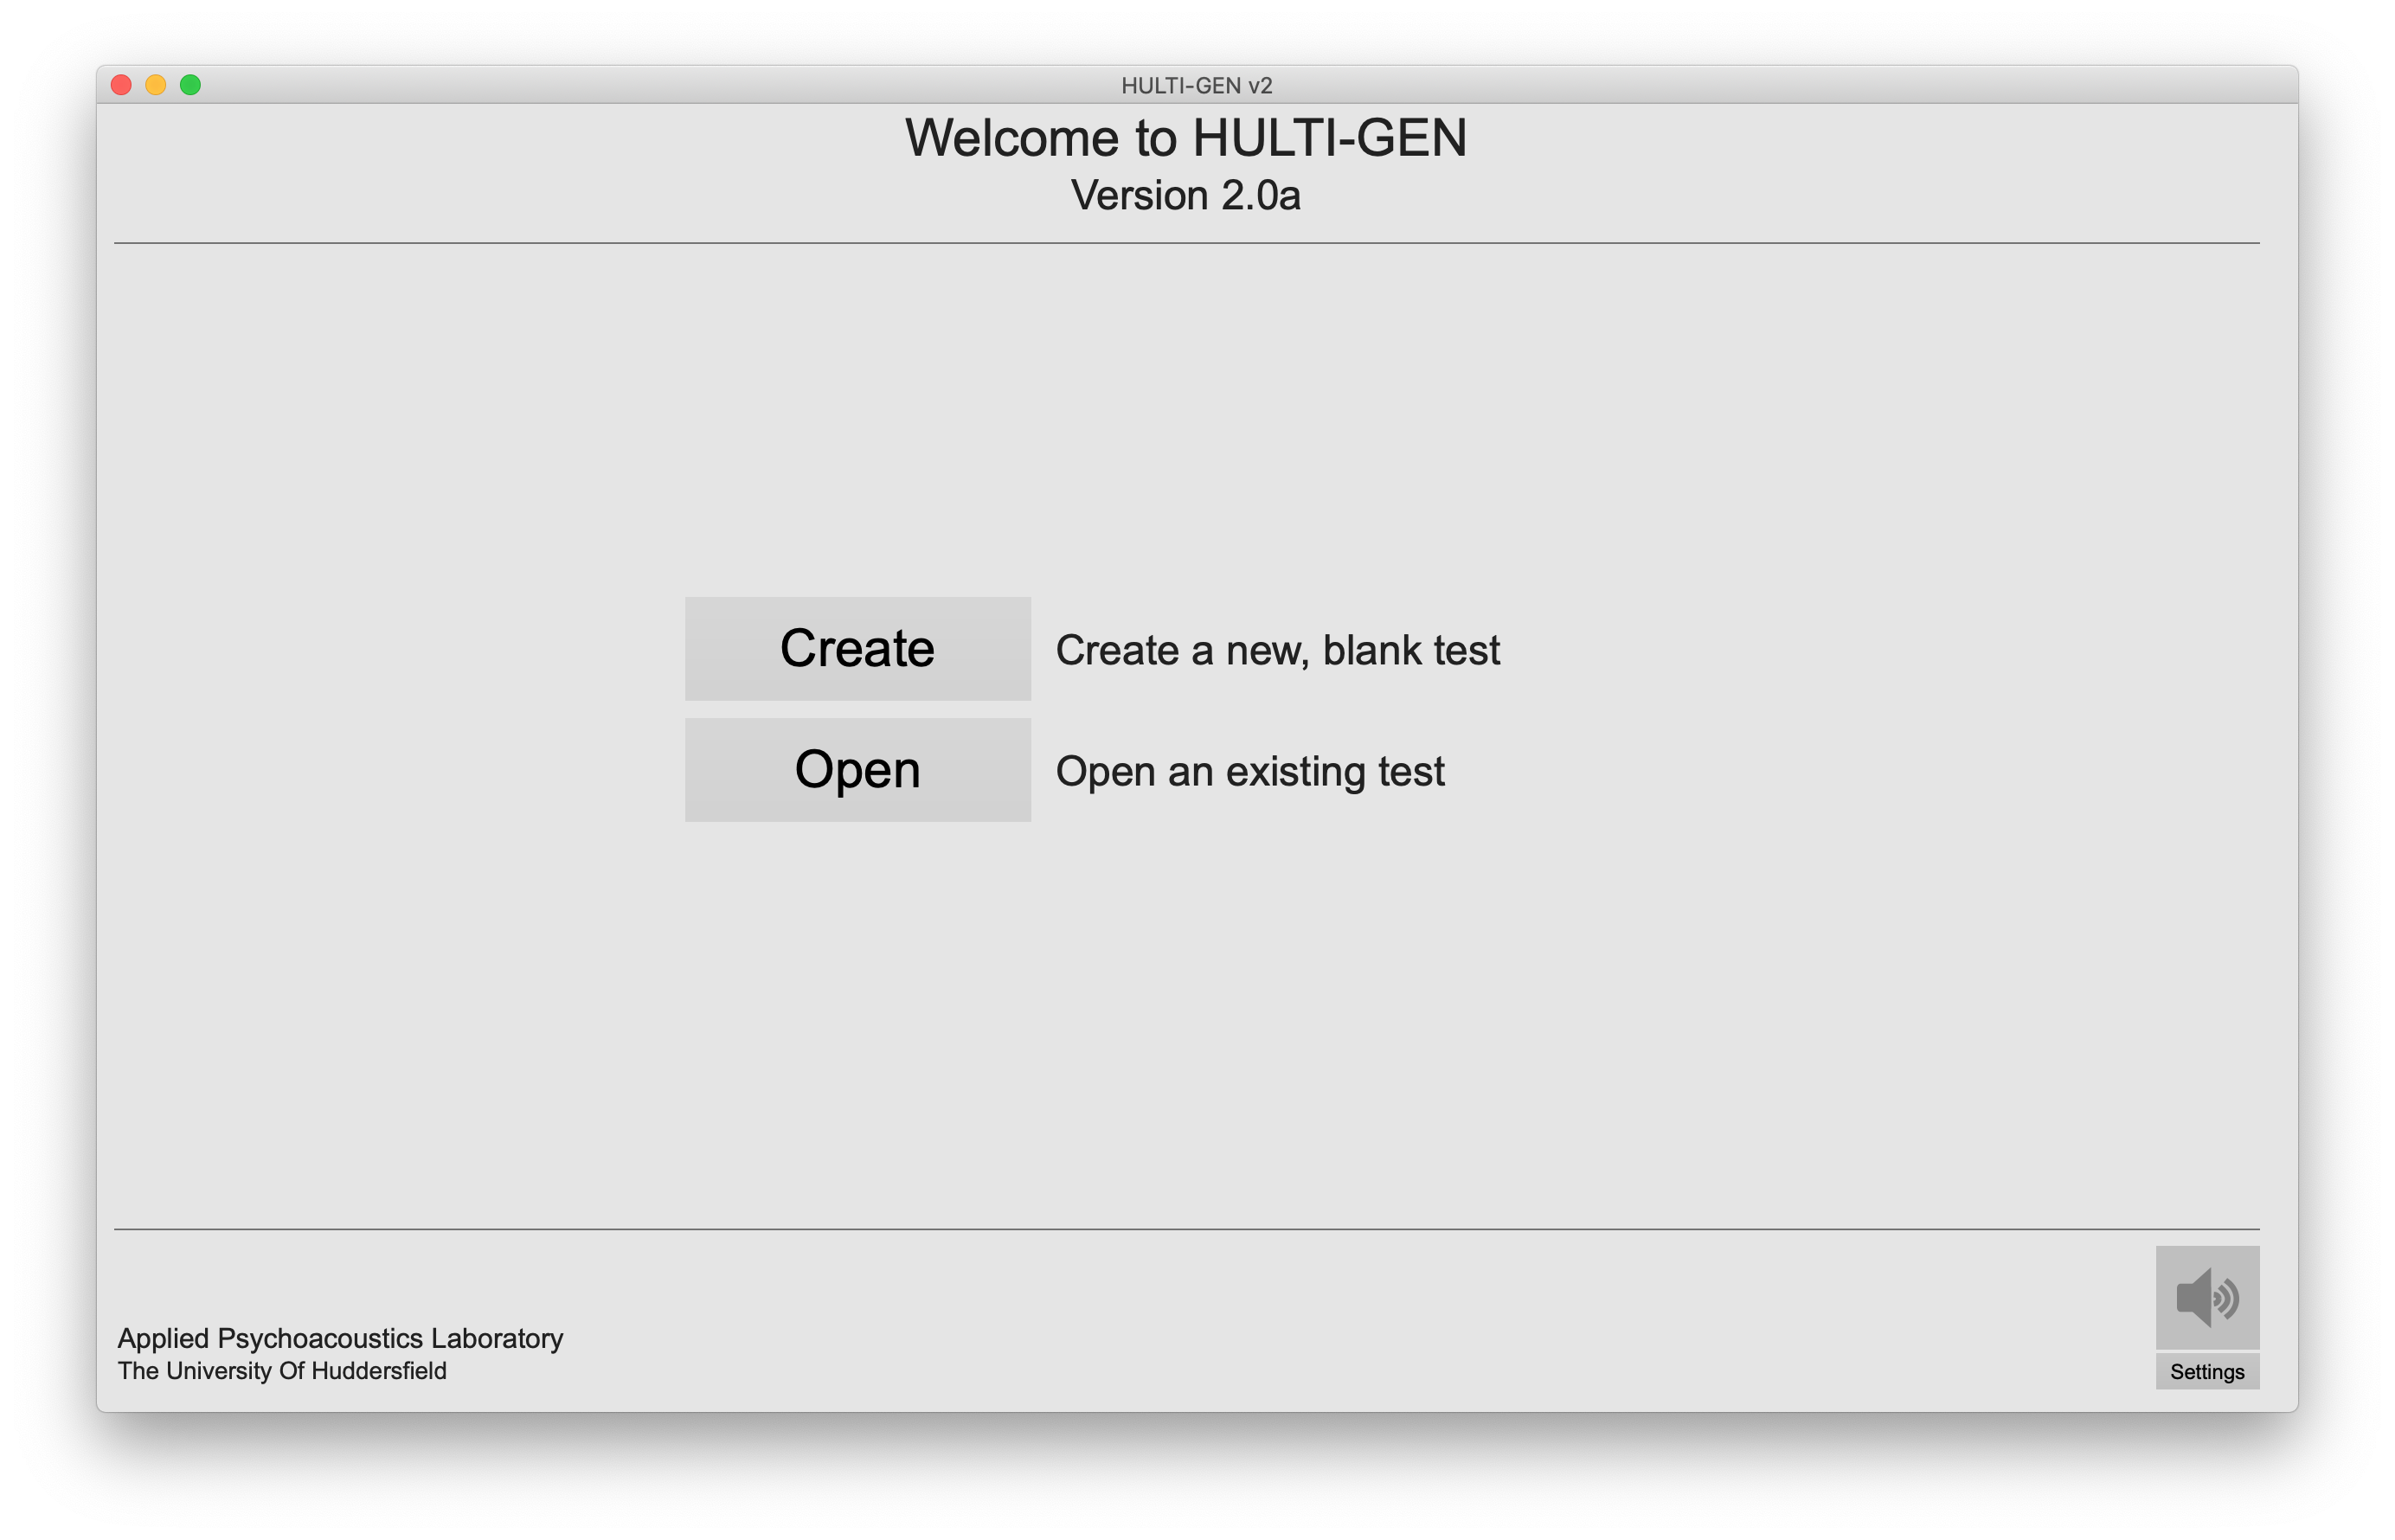
\includegraphics[width=1.0\textwidth]{./images/createTest_step01_mainScreen.png}
	\caption{Click on the 'Create' button to begin the test setup assistant.}
	\label{mainScreen}
\end{figure}
\pagebreak

\section{Creating a new test}
HULTI-GEN provides a step-by-step, test creation setup assistant. This assistant guides you through selecting a test method appropriate for your experiment, setting the parameters for your chosen method, customising the interface\footnote{Currently only available for grading tests}, adding stimuli, and assigning the stimuli into sessions and groups.
\newline\newline
From the main menu, click the 'Create' button to create a new test and begin the setup assistant. In each step of the setup process, you will be greeted by settings or options for that step. Once you have completed a step, click on the 'Next' button to move onto the next step.

\subsection{Step 1 - Choose a test method}
When you begin creating a new test, you will be asked what kind of test method, or task, you want subjects to perform, see Figure \ref{create::chooseTest}.

\begin{figure}[ht]
	\centering
	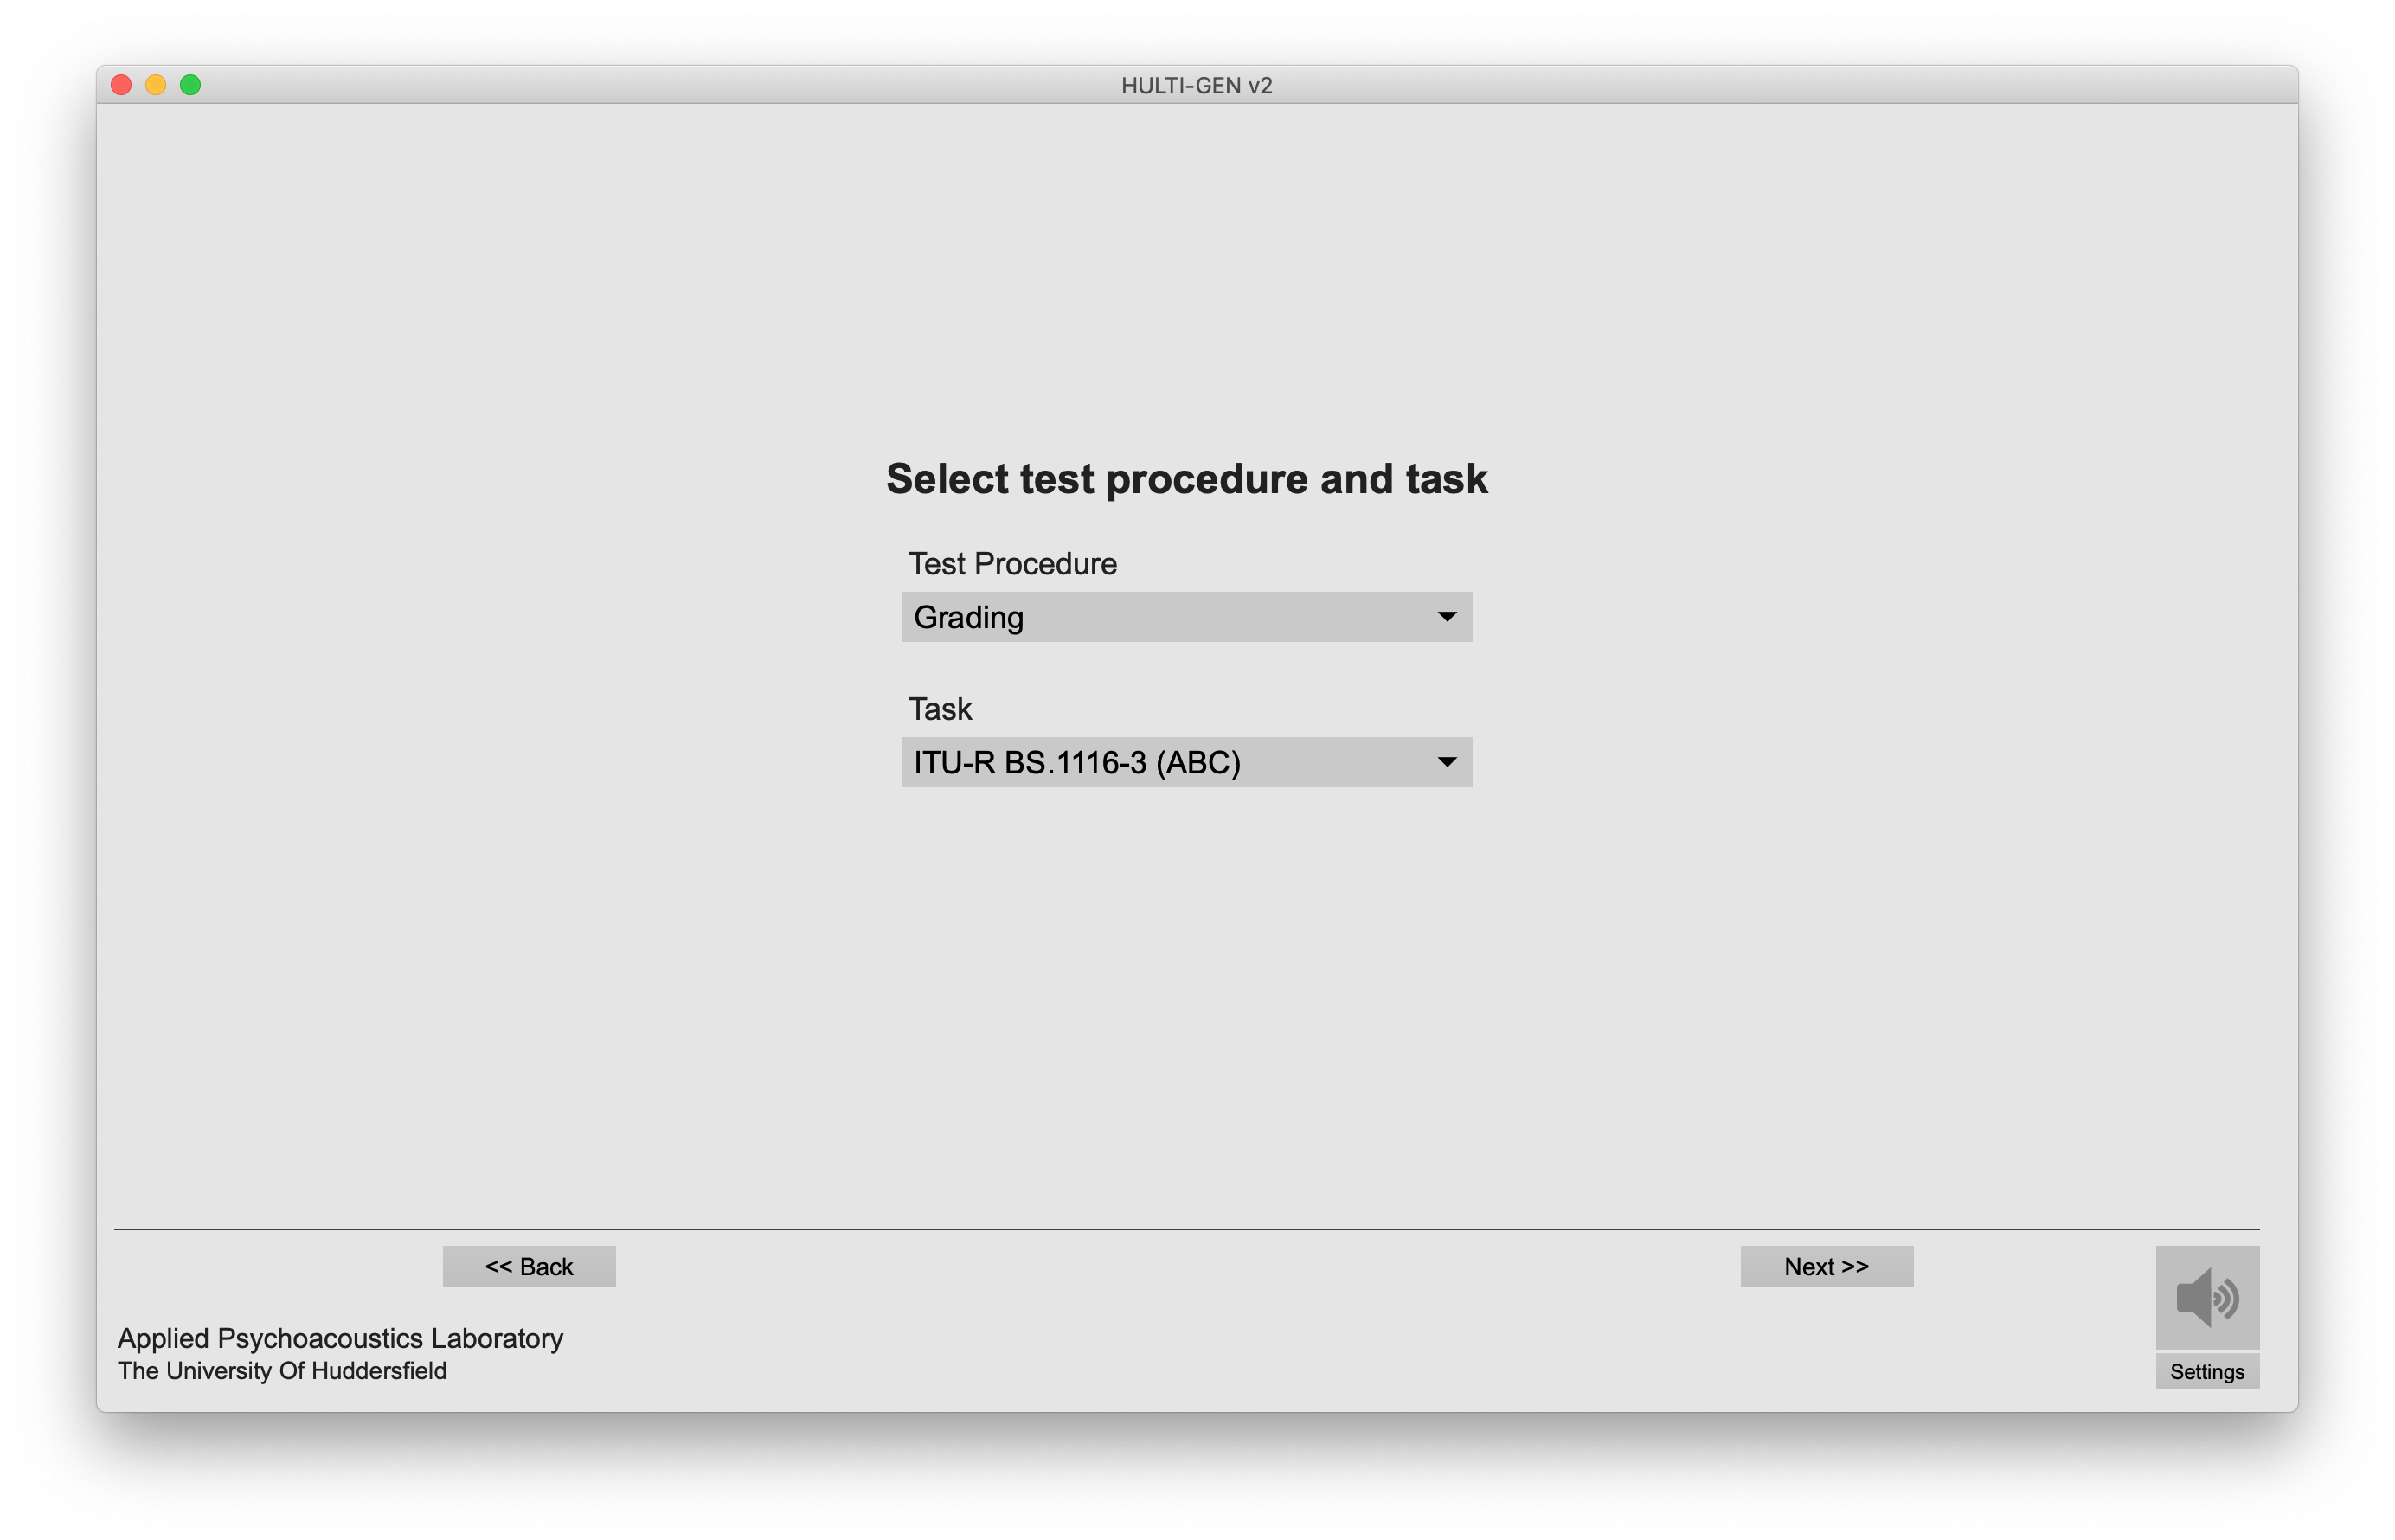
\includegraphics[width=1.0\textwidth]{./images/createTest_step02_chooseTest.png}
	\caption{Choose what type of procedure and task from the on-screen drop-down menus.}
	\label{create::chooseTest}
\end{figure}
\noindent
Each test method available in HULTI-GEN is grouped by \emph{Procedure} and \emph{Task}. Procedure groups each task by its testing process. Task is specific task the subjects will carry out during the experiment, e.g. MUSHRA. The following table lists all available tasks grouped by their corresponding procedures. Once you have selected a task, click 'Next'.

\begin{center}
	\begin{tabularx}{\textwidth}{|c|X|}
		\hline
		\textbf{Procedure} & \textbf{Task} \\
		\hline
		\multirow{7}*{Grading}
		& ITU-R BS.1116-3 (ABC)\\
		& ITU-R BS.1534-3 (MUSHRA)\\
		& Bipolar $\pm$50 with reference\\
		& ITU-T P.910 Absolute Category Rating (ACR)\\
		& ITU-T P.800 Degradation Category Rating (DCR)\\
		& ITU-T P.800 Comparison Category Rating (CCR)\\
		& 9-Point Hedonic Scale\\
		\hline
		\multirow{6}*{Non-Adaptive Psychophysical}
		& Two-Alternative Forced-Choice (2AFC)\\
		& ABX\\
		& Yes-No\\
		& Signal Detection Theory 2AFC\\
		& Signal Detection Theory ABX\\
		& Signal Detection Theory Yes-No\\
		\hline
		\multirow{3}*{Adaptive Psychophysical}
		& Staircase 2AFC\\
		& Staircase ABX\\
		& Staircase Yes-No\\
		\hline
	\end{tabularx}
\end{center}

\subsection{Step 2 - Input test parameters} 

On this screen you can set the number of sessions, or sittings, and groups of stimuli for the entire test.

\begin{figure}[ht]
	\centering
	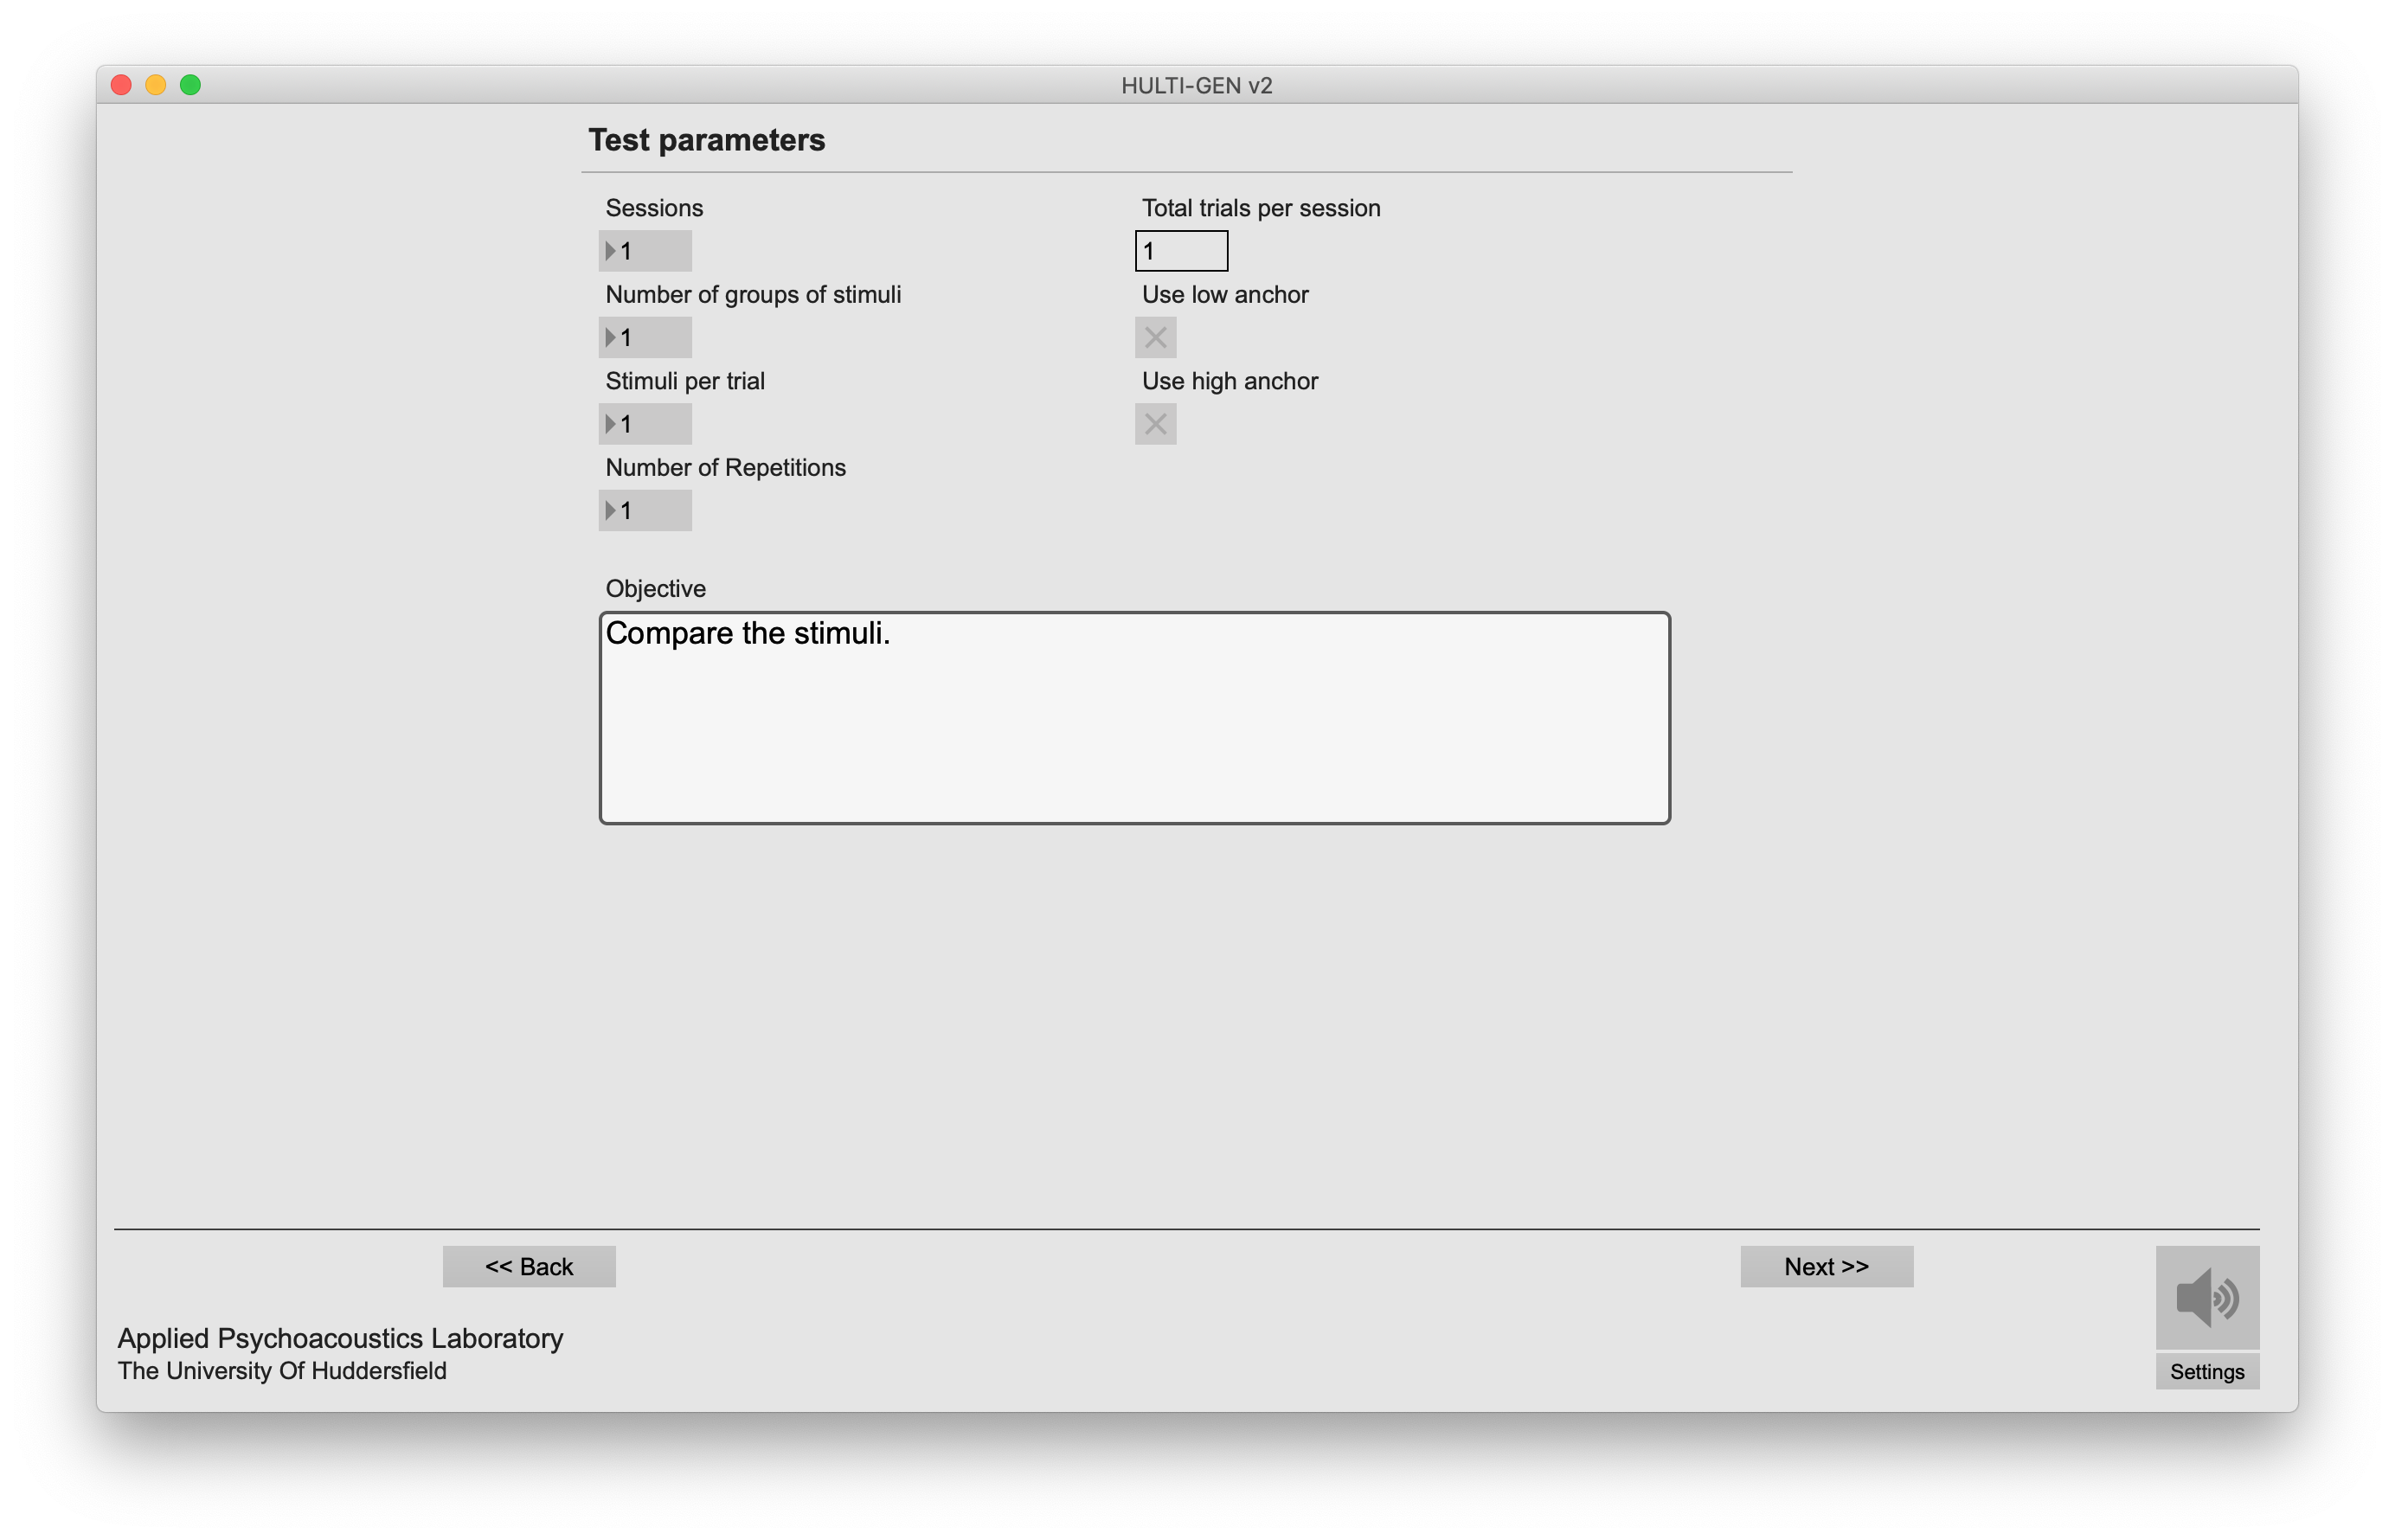
\includegraphics[width=1.0\textwidth]{./images/createTest_step03_testSettings.png}
	\caption{Example test parameters screen.}
	\label{create::testSettings}
\end{figure}

The type settings that you will see are contextual, whereby they depend on the type of procedure that you are configuring. The following list of descriptions explain the settings common to all procedures.

\begin{description}
	\item[Sessions] The number of sittings a subject will undertake for the entire test
	\item[Number of groups of stimuli] Sets the number of stimulus groups per session. In grading tests, this also sets the base number of trials.
	\item[Objective] The instructions that the subject will be shown on screen during the test.
\end{description}

\noindent
\textit{\textbf{Warning:} If at any point in setup process the number of sessions / groups are changed after being set, assignment of stimuli to any now non-existent sessions / groups will be destroyed.}

\subsection{Step 3 - Customise the test interface}

In this step you are able to customise various aspects of the test interface\footnote{\textit{\textbf{Note:} The customisation step is currently only available for grading tasks. Customisation will be made possible for all built-in procedures and tasks in future updates to HULTI-GEN}}. You can edit and resize the labels, change the scale minimum / maximum points and resolution, and (if enabled) position the high and low anchor buttons.

\begin{figure}[ht]
	\centering
	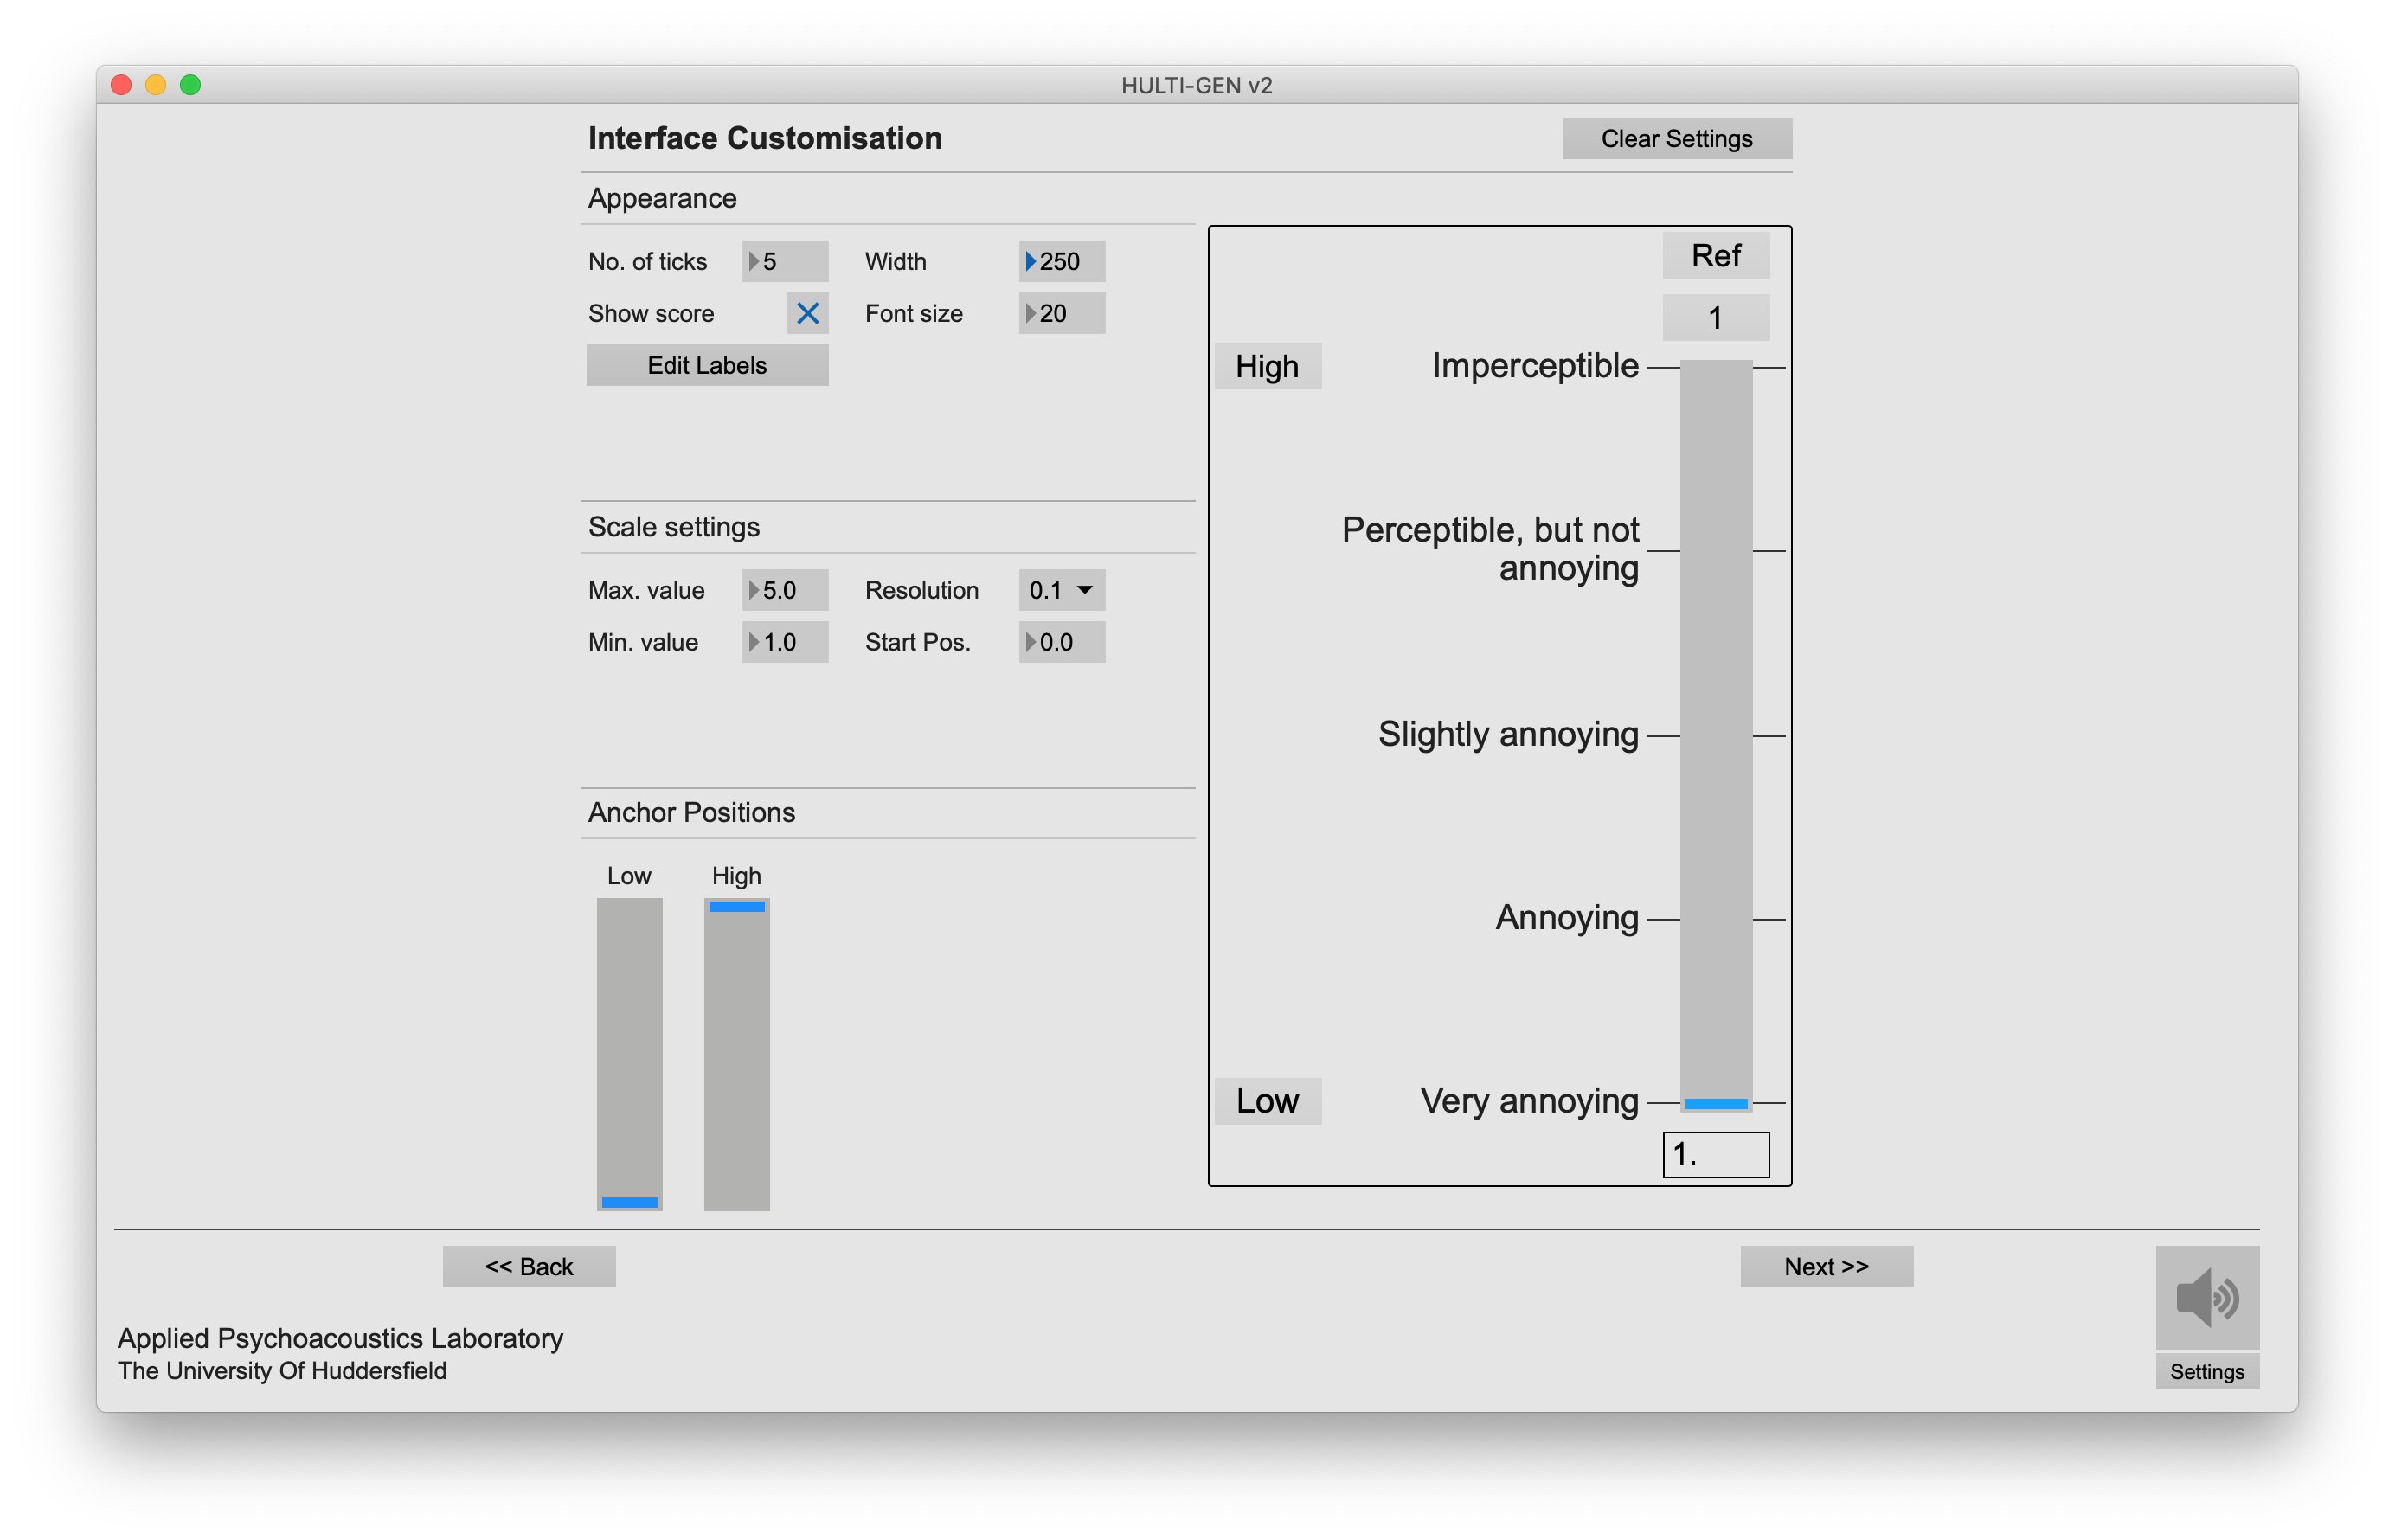
\includegraphics[width=1.0\textwidth]{./images/createTest_step04_customisation.png}
	\caption{Customise the test interface to suit the needs of your experiment.}
	\label{create::customisation}
\end{figure}

\noindent
By default the interface is set to follow the recommendations for the chosen task. Therefore, customising the testing interface means you are working outside of the recommendation. This is not a discouragement, but a reminder that you should justify the design of your test interface where required. After all, the aim of HULTI-GEN is allow experimenters to invent and try new ideas.

\subsection{Step 4 - Load stimuli}
Now that the test parameters have been set, it is now time load stimuli. First, the stimuli need to be loaded into a \emph{pool}, which is collection of all the stimuli used throughout the entire test.
\newline\newline
\textit{\textbf{Warning:} Due to the method of how Max locates files and dependencies, stimulus files \textbf{must} be placed in the HULTI-GEN folder or next to the application file (HULTI-GENv2.maxproj) \textbf{before running HULTI-GEN}, otherwise Max will not be able to find and load your stimuli files}.

\begin{figure}[ht]
	\centering
	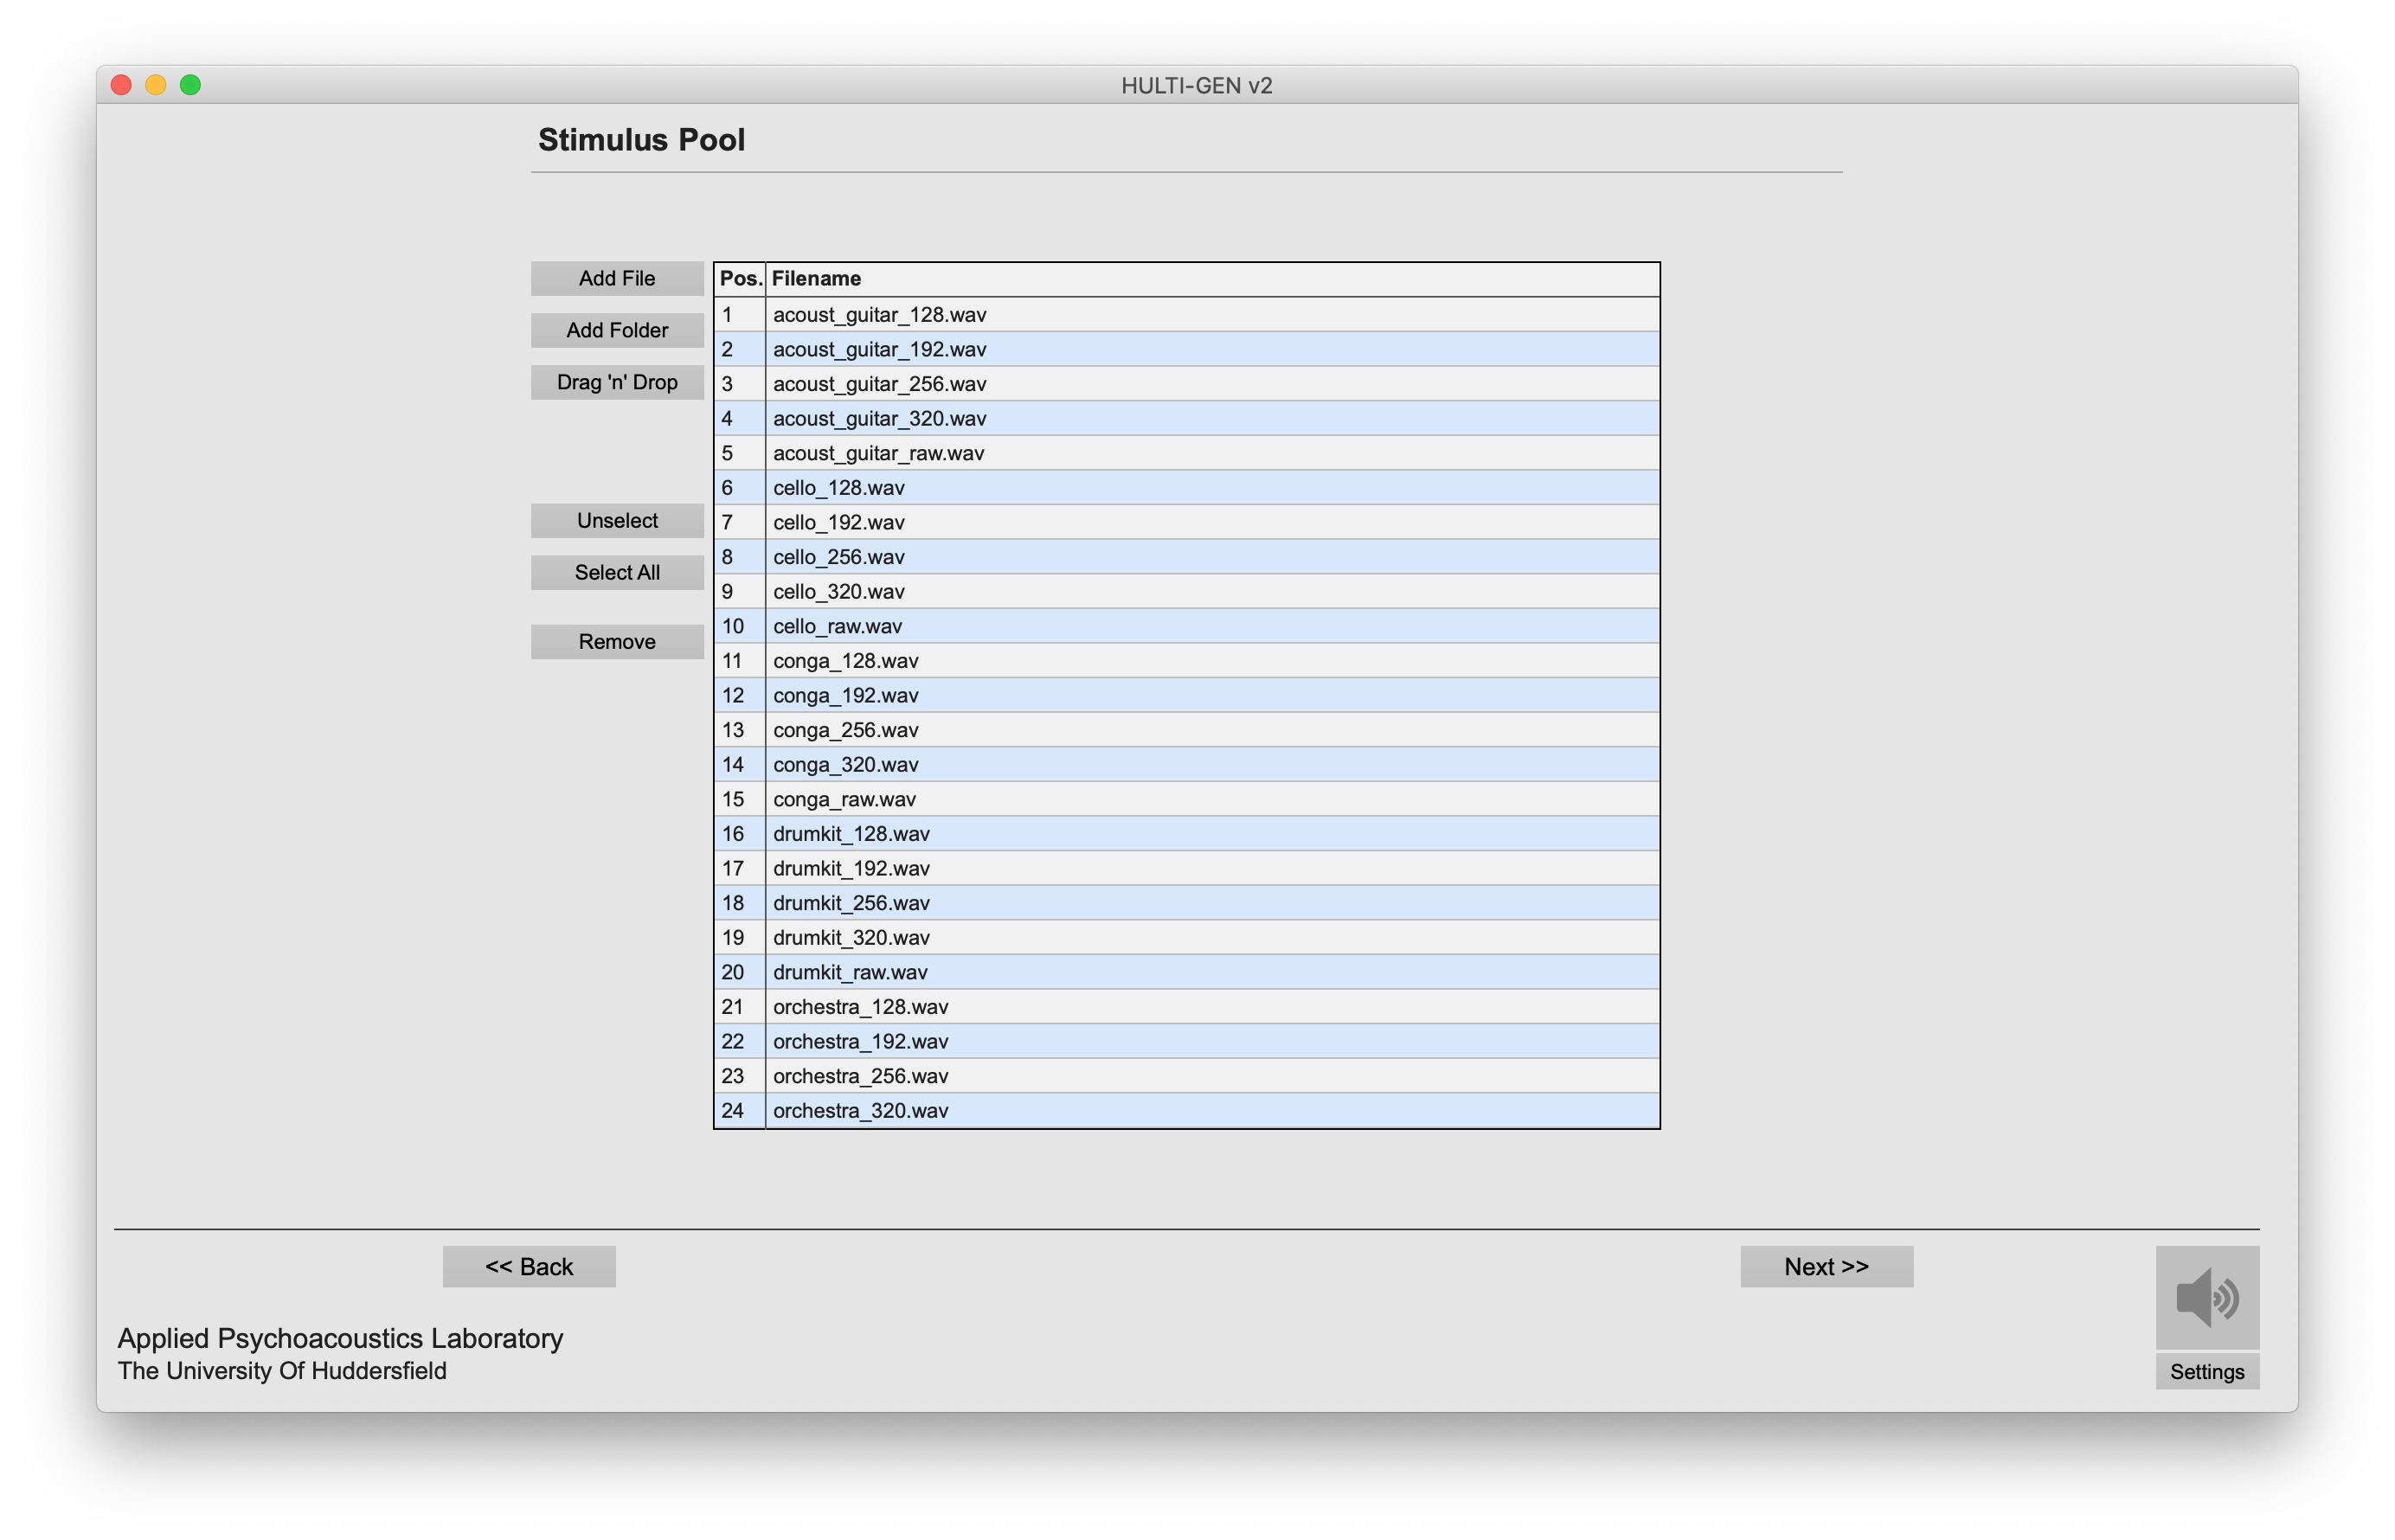
\includegraphics[width=1.0\textwidth]{./images/createTest_step05_stimulusPool.png}
	\caption{Stimuli for the entire test are loaded into a \emph{pool} using this interface.}
	\label{create::stimulusPool}
\end{figure}

\noindent
There are three main ways to add stimuli to the pool.
\begin{description}
	\item[Add File] Browse for and add individual files.
	\item[Add Folder] Browse for and an entire folder of files.
	\item[Drag 'n' Drop] Enable the drag and drop feature of the file-list. When enabled, you can drag files directly onto the file-list, where they are then appended to the list.
\end{description}

\noindent
As you load stimuli into the pool, their filenames are displayed in the file-list in the middle of the screen. Stimuli can be remove by first selecting items in the list, then click 'Remove'. You can select multiple items in the list by holding down 'Cmd' / 'Ctrl' (Operating System dependent) or 'Shift', much like the file browser built into your Operating System.
\pagebreak

\subsection{Step 5 - Assign stimuli}
The final step of the setup assistant is assigning stimuli to each session and group. This screen is divided into three main parts: Session and group menu, stimulus pool, and group sub-pool. Once all groups have been assigned stimuli, clicking 'Finish' will complete the process and take you to the 'Test menu'.

\begin{figure}[ht]
	\centering
	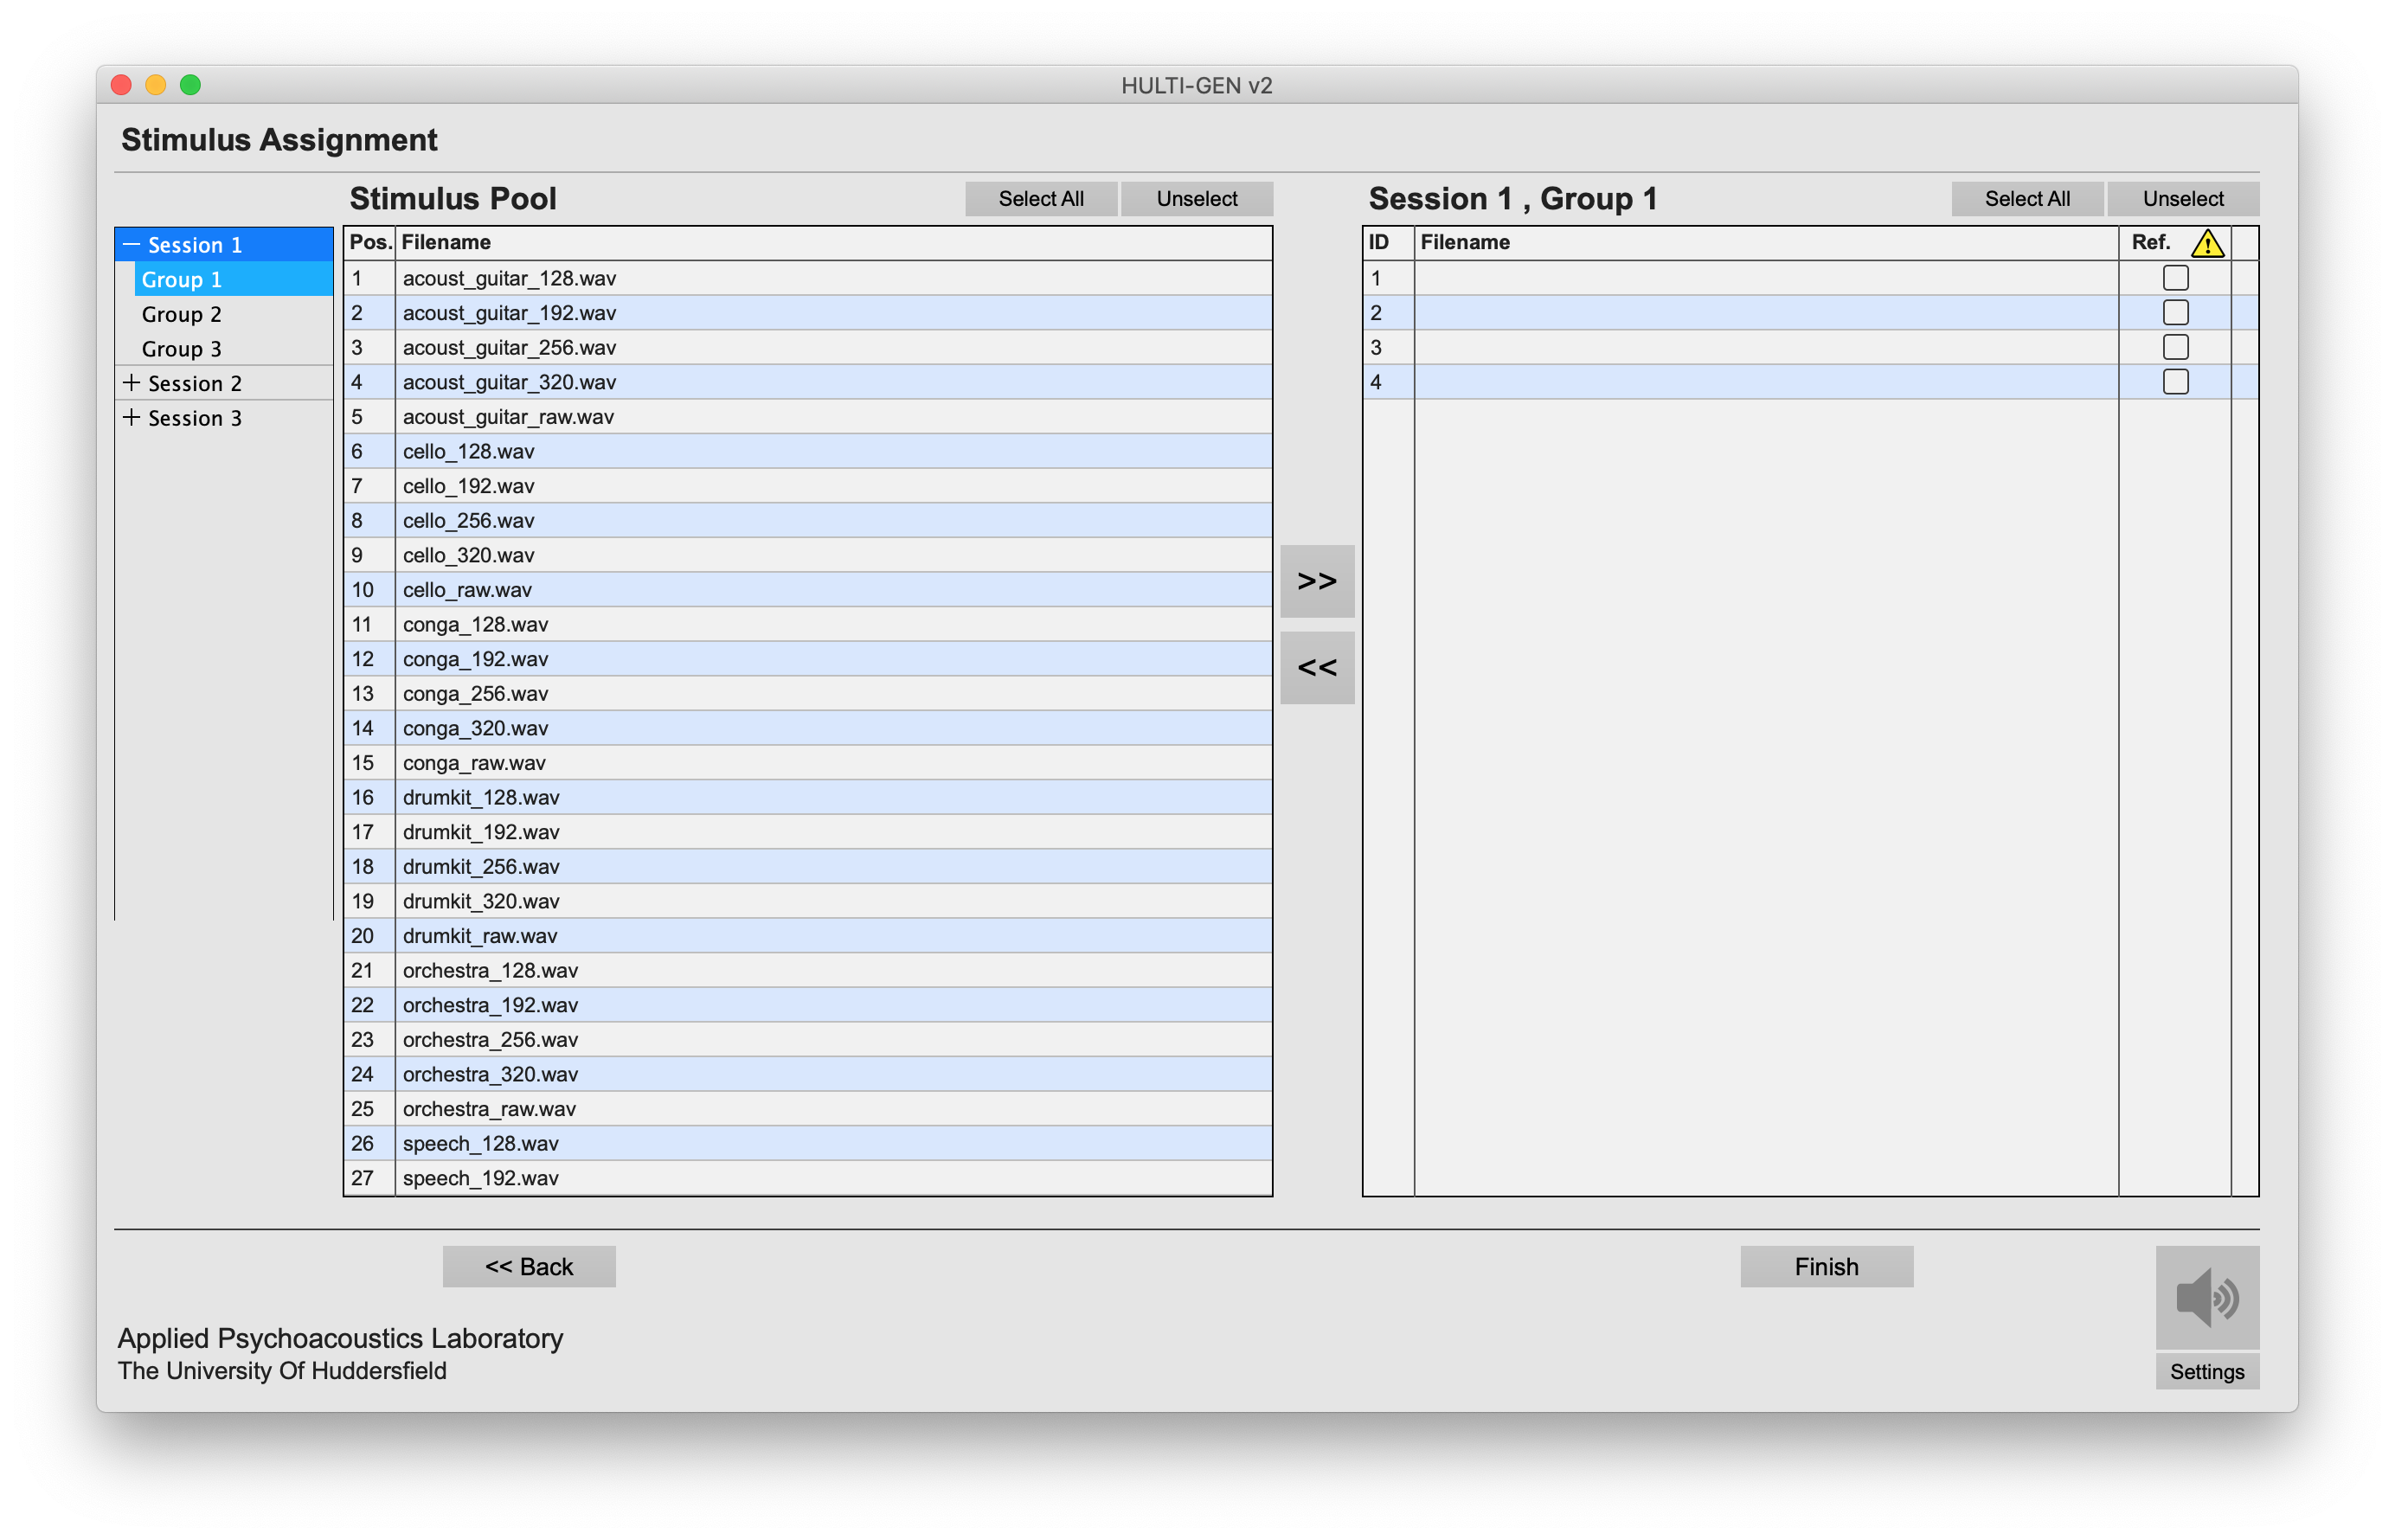
\includegraphics[width=1.0\textwidth]{./images/createTest_step06_stimulusAssign.png}
	\caption{The stimulus assignment screen. Stimuli in the pool on the left can be assigned to a group on the right.}
	\label{create::stimulusAssign}
\end{figure}

\subsubsection{Assigning to a group}
To assign stimuli to a group:
\begin{enumerate}
	\item Select a session and a group in the left-hand menu.
	\item Highlight your desired stimuli in the \emph{Stimulus Pool}
	\item Press the '$>>$' button to assign the stimuli to that group. They will then appear in the group sub-pool list on the right.
\end{enumerate}

\subsubsection{Removing from a group}
To remove stimuli from a group:
\begin{enumerate}
	\item Highlight the stimuli to remove in the group sub-pool list.
	\item Press the '$<<$' button to remove the highlighted stimuli from that group.
\end{enumerate}

\subsubsection{Grading test reference and anchor assignment}
Certain grading tests in HULTI-GEN require a reference stimulus, and if specified, also require 'Low' and 'High' anchors. A stimulus is set as a reference or anchor by checking the relevant checkbox in right most columns.

\begin{figure}[ht]
	\centering
	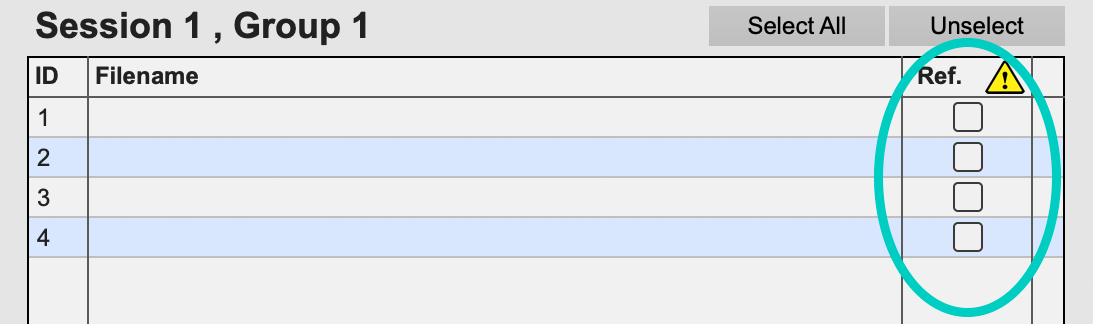
\includegraphics[width=0.8\textwidth]{./images/createTest_step06_anchorCheck.png}
	\caption{A stimulus is set as a reference or anchor by checking the relevant checkbox.}
	\label{create::stimulusAssignCheck}
\end{figure}

\subsubsection{Staircase step definition}
If you are configuring a staircase test, the position of the stimulus in the list determines which step of the staircase it is assigned to. By default the staircase tests begin at the highest level, which is the highest \emph{numbered} positions of the list, which is marked \emph{Maximum difference}, see Figure \ref{create::staircase}. This is may seem little confusing at first, but essesntially the list represents the staircase upside-down. The general rule is to assign the reference stimulus at position 1, or the \emph{Reference} position, and work down the list with increasing stimulus levels until you reach the stimulus that has the \emph{Maximum difference} compared to the reference.

\begin{figure}[ht]
	\centering
	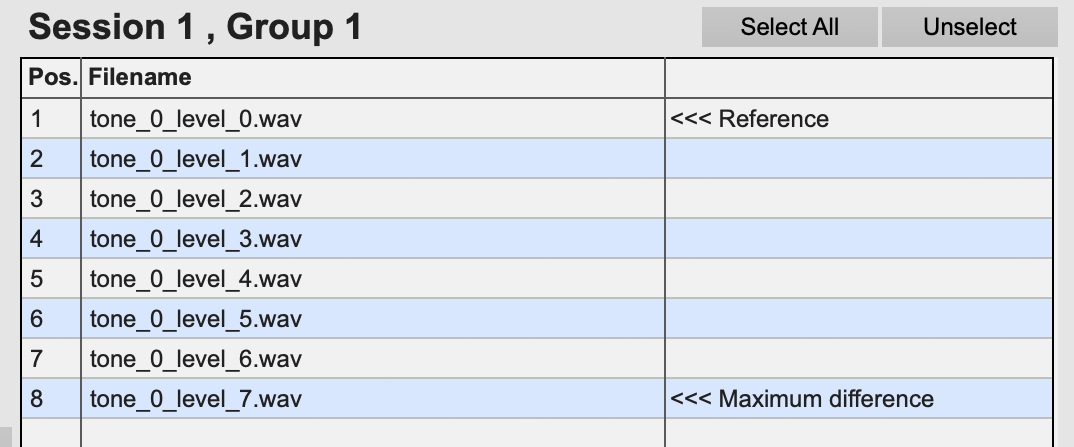
\includegraphics[width=0.8\textwidth]{./images/createTest_step06_staircase.png}
	\caption{Stimuli are arranged from the \emph{bottom}, reference step to the \emph{top}, maximum difference step.}
	\label{create::staircase}
\end{figure}


\chapter{Running a test}
\chapter{Audio settings}
Version 2.0 of HULTI-GEN features a multi-channel audio playback engine featuring real-time binauralisation and headphone filtering. This engine takes advantage of the MC, or Multi-Channel, processing that was introduced in Max 8, and supports up to 64-channels of multi-channel audio playback\footnote{Whilst it is possible to process up to 1024 channels of audio in Max 8, for technical reasons in HULTI-GEN it has been limited to 64 channels.}. The settings for the audio engine are accessed by clicking on 'Settings' under the speaker icon at the bottom-right corner of HULTI-GEN.

\begin{figure}[h]
	\centering
	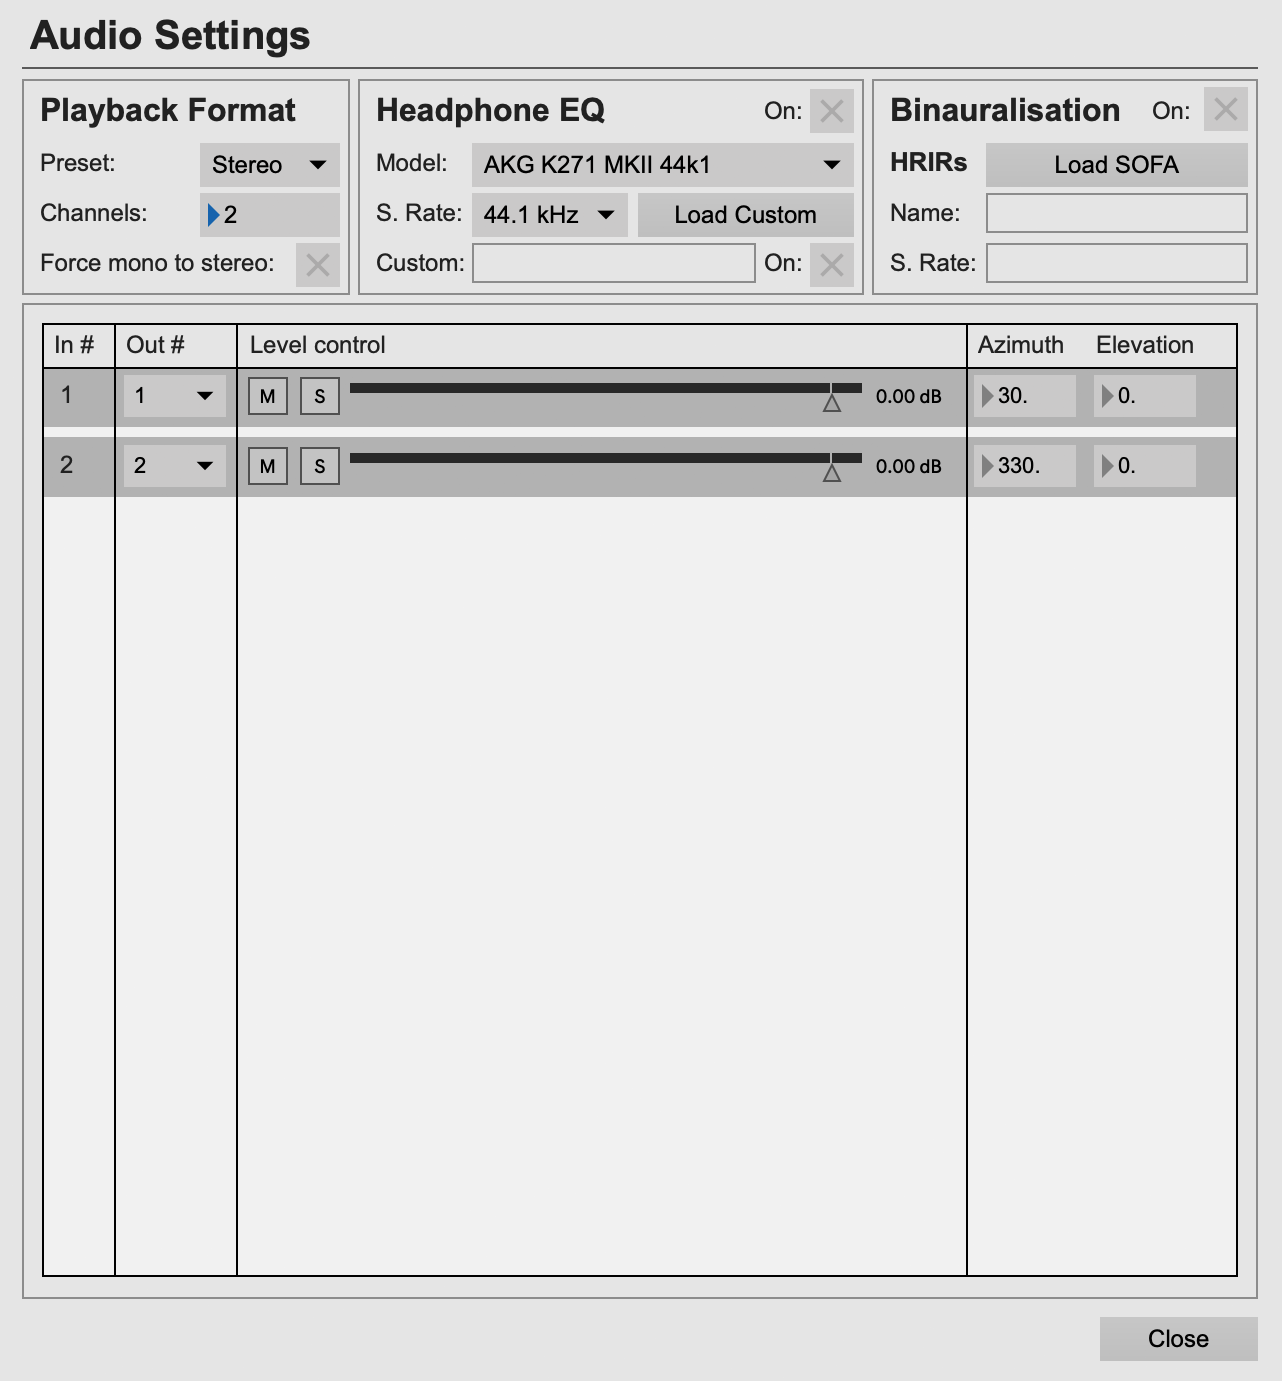
\includegraphics[width=0.7\textwidth]{./images/audioSettings_main.png}
	\caption{Audio settings screen.}
	\label{audioSettings::main}
\end{figure}

\noindent
The audio settings screen is split into four main parts: 'Playback Format', 'Headphone EQ', 'Binauralisation', and the channel list.

\section{Playback format}
The 'Playback Format' section allows you to define the number of output channels you will be using in you test, and is linked to the channel list. Here is a summary of the controls in this section:
\begin{description}
	\item[Preset] Set the channel list and 'Binauralistion' virtual speaker layout to one of the built-in configurations, e.g. 2.0, 5.0, 9.0 etc.
	\item[Channels] Sets the number of channels that will be used in the audio stream.
	\item[Force mono to stereo] Copies channel 1 to channel 2 for when you are using a mono stimuli but wish to use 2 a channel stereo loudspeaker setup or headphones.
\end{description}

\section{Headphone equalisation}
If you are using headphones for your test, it is sometimes desirable to reduce or \emph{cancel out} the effect of the headphone's own frequency response. The 'Headphone EQ' section allows you to apply headphone equalisation, either by using a matching, built-in, EQ filter, or by loading your own filter. The following is a summary of the controls in this section:
\begin{description}
	\item[Model] Selects which of the built-in headphone equalisation filter you want to use.
	\item[Load Custom] Allows you to load your own measured, headphone EQ, inverse filter.
	\item[Custom] This text box displays the filename of your custom filter. 
\end{description}
\noindent
The equalisation is enabled by toggling the top 'On' switch, whilst the custom filter is used in place of the built-in filter by toggling the 'On' switch next to the 'Custom' filename box.
\linebreak\linebreak
\noindent
\textit{\textbf{Warning:} The current version of HULTI-GEN does not feature any form of resampling of headphone EQ filters. Therefore, it is crucial that you the sample-rate of your chosen filter matches the sample-rate of Max or vice-versa.}

\section{Binauralisation}
Finally, the 'Binauralisation' section allows you to convert each audio channel into a virtual loudspeaker. The position of this virtual loudspeaker is set by the 'Azimuth' and 'Elevation' number boxes in the channel list. This process requires a Head Related Impulse Response (HRIR) database in the form of a SOFA file. These files are available from the internet. The following list describes the controls for this section:
\begin{description}
	\item[Load SOFA] Opens a dialog that lets you browse for and load a SOFA file. Binauralisation is only possible once a SOFA file has been loaded.
	\item[Name] Displays the filename of the currently loaded SOFA file.
	\item[S. Rate] Abbreviation of sample-rate, displays the sample-rate of the SOFA file.
\end{description}

\noindent
\textit{\textbf{Warning:} The current version of HULTI-GEN does not feature any form of resampling of HRIRs. Therefore, it is crucial that you the sample-rate of your chosen SOFA file matches the sample-rate of Max or vice-versa.}

\appendix
\chapter{CSV results file format}

\section{Individual subject CSV files}

Once a subject has completed all sessions in a test, HULTI-GENv2 will prompt the user to save a 'Comma Separated Values' (.CSV) file. This file is saved in conjuction with the subject's .JSON file, and is supported by most statistical analysis and speadsheet applications. The data in each column of a CSV file is formatted in hierarchical fashion, depending on the procedure. For grading and non-adaptive psychophysical tests, e.g. 1534-2 MUSHRA, MoC 2AFC etc, the hierarchy is:

\begin{center}
	\textbf{Session $\rightarrow$ Group $\rightarrow$ Stimulus $\rightarrow$ Repetition $\rightarrow$ Response / Grading Value}
\end{center}
\noindent
Whilst for adaptive methods, e.g. Staircase 2AFC, the hierarchy is:

\begin{center}
	\textbf{Session $\rightarrow$ Group $\rightarrow$ Trial $\rightarrow$ Step / Stimulus $\rightarrow$ Response}
\end{center}
\pagebreak
The following table is an example of a subject's CSV file for a 1534-2 MUSHRA, grading test arranged as 2 Sessions, 2 Groups, 3 Stimuli per Group repeated 2 times:

\begin{center}
	\begin{tabularx}{\textwidth}{|X|X|X|X|X|}
		\hline
		\textbf{Session ID} & \textbf{Group ID} & \textbf{Stimulus} & \textbf{Repetition} & \textbf{Response} \\
		\hline
		0 & 0 & 0 & 0 & 100. \\
		0 & 0 & 0 & 1 & 100. \\
		0 & 0 & 1 & 0 & 97. \\
		0 & 0 & 1 & 1 & 98. \\
		0 & 0 & 2 & 0 & 50. \\
		0 & 0 & 2 & 1 & 45. \\
		\hline
		0 & 1 & 0 & 0 & 100. \\
		0 & 1 & 0 & 1 & 100. \\
		0 & 1 & 1 & 0 & 86. \\
		0 & 1 & 1 & 1 & 90. \\
		0 & 1 & 2 & 0 & 31. \\
		0 & 1 & 2 & 1 & 38. \\
		\hline
		1 & 0 & 0 & 0 & 100. \\
		1 & 0 & 0 & 1 & 100. \\
		1 & 0 & 1 & 0 & 90. \\
		1 & 0 & 1 & 1 & 89. \\
		1 & 0 & 2 & 0 & 44. \\
		1 & 0 & 2 & 1 & 40. \\
		\hline
		1 & 1 & 0 & 0 & 100. \\
		1 & 1 & 0 & 1 & 100. \\
		1 & 1 & 1 & 0 & 75. \\
		1 & 1 & 1 & 1 & 78. \\
		1 & 1 & 2 & 0 & 20. \\
		1 & 1 & 2 & 1 & 25. \\
		\hline
	\end{tabularx}
\end{center}

\pagebreak
The following table is an example of a subject's CSV file for an Adaptive Staircase 2AFC test arranged as 2 Sessions and 2 Groups per session (\textit{\textbf{Note:} For clarity, the table has been truncated}):

\begin{center}
	\begin{tabularx}{\textwidth}{|X|X|X|X|X|}
		\hline
		\textbf{Session ID} & \textbf{Group ID} & \textbf{Trial} & \textbf{Step} & \textbf{Response} \\
		\hline
		0 & 0 & 0 & 10 & 1 \\
		0 & 0 & 1 & 10 & 1 \\
		0 & 0 & 2 & 9 & 1 \\
		0 & 0 & 3 & 9 & 1 \\
		0 & 0 & 4 & 8 & 1 \\
		0 & 0 & 5 & 8 & 1 \\
		0 & 0 & 6 & 7 & 1 \\
		0 & 0 & 7 & 7 & 1 \\
		0 & 0 & 8 & 6 & 1 \\
		0 & 0 & 9 & 6 & 1 \\
		0 & 0 & 10 & 5 & 1 \\
		0 & 0 & 11 & 5 & 0 \\
		0 & 0 & 12 & 6 & 0 \\
		0 & 0 & 13 & 7 & 1 \\
		0 & 0 & 14 & 7 & 1 \\
		0 & 0 & 15 & 6 & 1 \\
		0 & 0 & 16 & 6 & 1 \\
		0 & 0 & 17 & 5 & 1 \\
		0 & 0 & 18 & 5 & 1 \\
		\vdots & \vdots & \vdots & \vdots & \vdots\\
		\hline
		0 & 1 & 0 & 10 & 1 \\
		0 & 1 & 1 & 10 & 1 \\
		0 & 1 & 2 & 9 & 1 \\
		0 & 1 & 3 & 9 & 1 \\
		0 & 1 & 4 & 8 & 1 \\
		0 & 1 & 5 & 8 & 1 \\
		0 & 1 & 6 & 7 & 1 \\
		0 & 1 & 7 & 7 & 1 \\
		0 & 1 & 8 & 6 & 1 \\
		0 & 1 & 9 & 6 & 1 \\
		0 & 1 & 10 & 5 & 1 \\
		0 & 1 & 11 & 5 & 0 \\
		0 & 1 & 12 & 6 & 1 \\
		0 & 1 & 13 & 6 & 1 \\
		0 & 1 & 14 & 5 & 1 \\
		0 & 1 & 15 & 5 & 1 \\
		0 & 1 & 16 & 4 & 1 \\
		0 & 1 & 17 & 4 & 1 \\
		0 & 1 & 18 & 3 & 1 \\
		\vdots & \vdots & \vdots & \vdots & \vdots\\
		\hline
	\end{tabularx}
\end{center}


% bibliography, glossary and index would go here.

\end{document}
